%!TEX encoding = UTF-8 Unicode

%!TEX root = ../compendium2.tex

\Lab{\LabWeekTEN}

\begin{Goals}
\item Kunna använda mönstermatchning.
\item Kunna förklara hur \code{Option} användas för att hantera saknde värden.
\item Känna till att \code{scala.util.Try} kan användas för att hantera undantag.
\item Känna till att undantag kan hanteras med \code{try catch}.

\end{Goals}

\begin{Preparations}
\item Gör övning {\texttt{\ExeWeekTEN}} i kapitel \ref{chapter:W10}.
\item Testa så att datorn du ska använda på redovisningen kan spela upp ljud med \code{javax.sound.midi} genom att köra igång \code{Main} i den givna koden.
\item Det är bra om du kan ta med hörlurar till laborationen så att du inte stör andra.
\end{Preparations}

\subsection{Bakgrund}
När man skriver program skapar man ofta modeller av en viss verklig \emph{domän}, som kan vara t.ex. försäkringskassans regelverk eller en fysiksimulering i ett datorspel. För att kunna skapa sådana modeller behöver man ofta skaffa sig  \emph{domänkunskap} genom att noga sätta sig in i vad olika koncept i domänen innebär och hur de är relaterade. Med denna kunskap kan du skapa kod som modellerar domänen, utifrån noga valda förenklingar av den komplexa verkligheten. Förmåga att kunna skapa domänmodeller utgör en viktig grund för konsten att utveckla bra programvarusystem, och du kommer lära dig mer om detta i kommande kurser.

I denna laboration ska du skapa ett program baserat på en förenklad modell av domänen \emph{musik}. Du får färdig kod som modellerar hur toner är uppbyggda, samt hur olika stränginstrument fungerar.
Med denna domänmodell ska du skapa ditt eget musikprogram som använder \emph{ackord} som är uppbyggda av flera toner som spelas tillsammans.

\subsection{Domänmodell}


\subsubsection{Tonhöjd}

En \textbf{ton} \Eng{note} som spelas på ett instrument, t.ex. ett piano eller en gitarr, har en \textbf{tonhöjd} \Eng{pitch} som är relaterad till den specifika  grundfrekvens som tonens ljud har. I vår modell av musikdomänen tillordnar vi olika distinkta tonhöjder ett unikt heltal. En tonhöjd kan då beskrivas av en \code{case class Pitch(nbr: Int)} där vi använder \code{nbr} i intervallet \code{(0 to 127)}. Heltalet \code{60} motsvarar en viss ton, som även har namnet  \code{"C5"}, och som ligger ungefär i mitten av tangentbordet på ett piano.

Inom (västerländsk) musik utgår man från 12 olika \emph{tonklasser} \Eng{pitch classes}.
Dessa tolv tonklasser är ordnade i en sekvens av så kallade \emph{halva tonsteg} och har följande \textbf{tonklassnamn}:
\begin{Code}
  val pitchClassNames: Vector[String] =
    Vector("C","C#","D","D#","E","F","F#","G","G#","A","A#","B")
\end{Code}
Efter tonklassen med namnet \code{B} återkommer tonklassen med namnet \code{C}.
Symbolen \code{#} representerar en höjning ett halvt tonsteg. Tonklassen \code{C#} uttalas \emph{siss} på svenska, och \emph{see sharp} på engelska.\footnote{Man använder även b-förtecknet $\flat$, som uttalas \emph{flat} på engelska, för sänkning av en ton ett halvt tonsteg, men för enkelhetens skull bortser vi i vår modell från detta sätt att namnge toner.}
 Notera att det är ett halvt tonsteg mellan \code{E} och \code{F}, samt mellan \code{B} och \code{C} (det finns därför varken \code{E#} eller \code{B#} i listan med tonklassnamn.\footnote{Varför det är på detta viset kan du läsa mer om på t.ex. Wikipedia, men du kan också nöja dig med att det helt enkelt är så på grund av historiska skäl.})

På ett piano motsvaras de vita tangenterna av tonklassnamen \code{C D E F G A B} och de svarta tangenterna motsvaras av tonklassnamnen \code{C# D# F# G# A#}.

En s.k. \textbf{tonklass} är ett positivt heltal i intervallet \code{0 until 12} som motsvaras av index för tonklassnamnet i \code{pitchClassNames}. En tonhöjd  \code{Pitch(nbr)} tillhör tonklassen \code{nbr % 12}.

Med hjälp av heltalsdivision med 12 får man fram tonhöjdens så kallade \textbf{oktav}, alltså \code{nbr / 12}. Ett piano har normalt toner som spänner över 7 eller 8 oktaver.
En tonhöjd \code{Pitch(nbr)} kan även namnges med en kombination av tonklassnamnet och tonens oktav, t.ex. \code{"C5"}.

Med denna domänbeskrivning kan vi skapa en mer detaljerad modell av konceptet tonhöjd med hjälp av en case-klass och tillhörande kompanjonsobjekt:

\scalainputlisting[basicstyle=\ttfamily\fontsize{10}{13}\selectfont]{../workspace/w10_music/src/main/scala/music/Pitch.scala}

\noindent Kompanjonsobjektet har två fabriksmetoder som kan skapa \code{Pitch}-objekt från en strängrepresentation av en tonhöjd.

\begin{itemize}[noitemsep]
  \item Metoden \code{fromString} omvandlar en sträng till en \code{Option[Pitch]}.

  \item Metoden \code {apply} kastar ett undantag om det inte går att omvandla en sträng till ett \code{Pitch}-objekt.
\end{itemize}

\Task\label{music:exceptions}\Pen Vilka två uttryck i \code{Try}-blocket kan ge undantag? Undersök liknande undantagsuttryck i REPL och skriv ner namnet på undantagen.


\Task Undersök klassen \code{Pitch} i REPL.

\begin{REPL}
> sbt
sbt> console
Welcome to Scala 2.12.3 (Java HotSpot(TM) 64-Bit Server VM, Java 1.8.0_144).

scala> import music._
import music._

scala> Pitch("C#5").nbr
res0: Int = 61

scala> Pitch("C") + 1
res1: music.Pitch = Pitch("C#5")
\end{REPL}


\Subtask\Pen Ge ett exempel på argument till \code{Pitch.apply} som gör att undantag kastas.

\Subtask\Pen Ge ett exempel på argument till \code{Pitch.fromString} som ger \code{None}.

\Subtask\Pen Ge ett exempel på argument till \code{Pitch.+} som gör att undantag kastas.


\Task Ändra i implementationen av \code{fromString} så att du i stället för \code{.toOption} gör en mönstermatchning med \code{match} på \code{Try}-resultaten \code{Success} och \code{Failure} i varsin case-klausul på formen \code{case Sucess(e) => } och \code{case Failure(e: ???) => ???} och returnera lämpligt värde. Ta endast hand om de två förväntade undantagstyperna som du identifierade i uppgift \ref{music:exceptions}. Gör så att alla övriga eventuella undantag kastas genom denna klausul: \code{case Failure(e) => throw e}

\Subtask Testa så att din lösning fungerar i både normalfall och vid felaktigt tönhöjdsnamn.

\Subtask\Pen Undersök vad som händer om du kommenterar bort olika case-klausuler. När ger kompilatorn varning? Varför?

\Subtask\Pen Finns det någon fördel resp. nackdel med att bara fånga vissa undantag?

\subsubsection{Ackord}

Ett ackord består av flera toner som spelas tillsammans. Man kan spela ett ackord på ett stränginstrument genom att slå an en mängd toner samtidigt eller en sekvens av toner i snabb följd. Man väljer att kalla en av tonerna i ackordet (oftast den lägsta/första tonen) för \textbf{grundton} \Eng{root}.

Ett \textbf{intervall} är en tons relativa tonhöjdsavstånd från grundtonen. Ackord har olika namn beroende på vilka intervall som ingår i ackordet. Det finns väldigt många olika ackordnamn, men här begränsar vi oss för enkelhetens skull till fyra olika typer av ackord: \footnote{Om du vill veta mer om ackordnamn läs här: \url{https://en.wikipedia.org/wiki/Chord_(music)}}
\begin{itemize}
  \item dur-ackord, betecknas t.ex. \code{"C"},
  \item moll-ackord, betecknas t.ex. \code{"Cm"}
  \item sju-ackord, betecknas t.ex. \code{"C7"}
  \item maj-sju-ackord som betecknas t.ex. \code{"Cmaj7"}.
\end{itemize}

I case-klassen \code{Chord} nedan finns en metod \code{name} som definerar vilka intervall som ingår i de olika ackordtyperna ovan, utom maj-sju-ackord. Den krångliga modulo-12-omräkningen innan matchningen gör så att intervall i olika oktaver behandlas lika, även för negativa intervall.

\scalainputlisting[basicstyle=\ttfamily\fontsize{10}{13}\selectfont]{../workspace/w10_music/src/main/scala/music/Chord.scala}

\Task

\Subtask Maj-sju-ackord har samma intervall som sju-ackord, förutom att det fjärde intervallet ska vara \code{11} halva tonsteg från grundtonen i stället för \code{10}. Lägg till en case-klausul i \code{Chord.name} så att maj-sju-ackord ges namn som slutar med ändelsen \code{"maj7"}.

\Subtask Testa din kod och kontrollera så att ackordet \code{Chord("D4","F#4","A4","C#5")} får namnet \code{"Dmaj7"}

\begin{REPL}
scala> Chord("D4","F#4","A4","C#5").name()
res2: String = "Dmaj7"
\end{REPL}

\Subtask Vilka fyra toner har ett \code{Cmaj7}-ackord med grundtonen \code{"C5"}?

\subsubsection{Stränginstrument}

Ett stränginstrument, t.ex. ett piano eller en gitarr, kännetecknas av att det kan spela ackord genom att flera strängar kan sättas i svängning så att många toner spelas tillsammans. I vår modell fångar vi denna egenskap med en trait \code{StringInstrument} som har en metod \code{toChordOpt} som ger något ackord om minst en sträng spelas.

Gitarr och ukulele är exempel på stränginstrument som har en greppbräda \Eng{fret board}. Man spelar på ett stränginstrument med greppbräda \emph{fretted instruments} genom att trycka strängar mot greppbrädan med en hand, samtidigt som man knäpper på strängarna med den andra handen. Olika instanser av dessa  instrument kan skilja sig åt vad gäller antalet strängar och hur dessa strängar är stämda. En normal gitarr har 6 strängar, medan en normal ukulele bara har 4 strängar. Dessa egenskaper modelleras i koden nedan.

Varje sträng har en stämskruv med vilken kan man ändra strängens spänning,  strängens s.k. \textbf{stämning} \Eng{tuning}.  Om man knäpper på alla lösa strängarna på en gitarr med standardstämning spelas tonerna E3, A3, D4, G4, B4, E5, räknat från den tjockaste till den tunnaste strängen.

\scalainputlisting[basicstyle=\ttfamily\fontsize{10}{12.9}\selectfont]{../workspace/w10_music/src/main/scala/music/instruments.scala}

Om man trycker på greppbrädans olika positioner får man olika toner, beroende på vilken position man trycker på. Positionerna på greppbrädan räknas från ett och uppåt. Position \code{0} motsvarar lös sträng. En negativ position, tex. \code{-1}, anger att en sträng inte spelas; många gitarrackord spelas genom att bara en delmängd av strängarna slås an.

Ett exempel på ett gitarrackord visas i figur \ref{music:fig:guitar-chord}. Detta motsvarar ackordet \code{Guitar(3,3,2,0,1,0)}, där tonen G spelas på den tjockaste strängen.

\Task\Pen Studera modellen av stränginstrument ovan och använd REPL för att svara på dessa frågor:

\Subtask Vad är namnet på detta pianoackord om vi väljer att lägsta tonen i ackordet är grundton: \code{Piano(Set(60, 64, 67, 70))}

\Subtask Vad heter tonerna som ingår i ackordet \code{Guitar(3,3,2,0,1,0)}.

\Subtask Vad heter detta ackord om vi väljer ett A som grundton: \code{ Ukulele(0,2,1,2)}


\begin{figure}
  \centering
  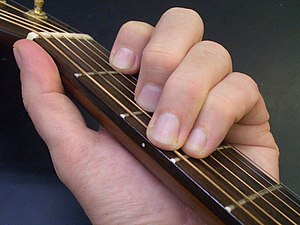
\includegraphics{../img/chords/guitar-C-major-chord.jpg}
  \caption{Ett C-dur-ackord på en gitarr med tonen G i basen.}
  \label{music:fig:guitar-chord}
\end{figure}


\subsubsection{Elektroniska instrument}

Ett elektroniskt instrument syntetiserar ljud med hjälp av analog och/eller digital elektronik, och kallas därför \textbf{synthesizer}, ofta förkortat \emph{synt} \Eng{synth}.

I JDK ingår ett api för att styra syntar. De flesta moderna datorer har ljudkort med inbyggd synt som följer den så kallade MIDI-standarden. Java-paketet \code{javax.sound.midi} innehåller klasser som kan få ett sådant ljudkort att spela musik med hjälp av MIDI.

MIDI-standarden baseras på en modell av ett pianotangentbord där olika toner kan vara ''på'' eller ''av'' beroende på om en tangent är nedtryckt eller ej. Dessa toners höjd är modellerade på samma sätt som i vår klass \code{Pitch}, där alltså tonhöjden \code{60} motsvarar tonen \code{"C5"}, etc. En tangent kan tryckas ner olika hårt, vilket representeras av ett heltalsvärde i \code{Range(0,128)} kallat \code{velocity}. Ett högt värde ger en stark ton, medan ett litet värde motsvarar en svag (tyst) ton.

En synt som följer MIDI-standarden kan spela upp ljud via 16 olika så kallade \textbf{kanaler} \Eng{channel}, numrerade \code{(0 until 16)},  där varje kanal kan ställas in så att den spelar ett ljud som t.ex. liknar ett visst verkligt instrument, så som piano eller gitarr.

I kursens workspace i paketet \code{music} finns en \code{Synth}-modul som förenklar användningen av Java-paketet \code{javax.sound.midi}. I modulen \code{Synth} finns metoden \code{playBlocking} som kan spela flera toner under en viss tid med hjälp av synten på ditt ljudkort. Exekveringen av ditt program  blockeras tills tonerna spelats klart, därav \emph{''blocking''} i namnet.

Metoden \code{playBlocking} har följande parametrar, default-argument och returtyp:
\footnote{Om du är nyfiken kan du studera implementationen av \code{Synth}-modulen här:
\\\url{https://github.com/lunduniversity/introprog/tree/master/workspace/w10_music}
 Koden blir lättare att förstå om du samtidigt läser api-dokumentationen av paketet \code{javax.sound.midi} och även lära dig mer om MIDI-standarden med hjälp av t.ex. wikipedia.}

\begin{Code}
def playBlocking(
  noteNumbers: Seq[Int] = Seq(60), // en sekvens av tonhöjder
  velocity: Int         = 60,      // hur hårt anslag i Range(0, 128)
  duration: Long        = 300,     // hur länge i millisekunder
  spread:   Long        = 50,      // millisekunder mellan tonerna
  after:    Long        = 0,       // millisekunder innan första tonen
  channel:  Int         = 0        // MIDI-kanal som spelar tonerna
): Unit
\end{Code}


\Task Anropa \code{playBlocking()} i REPL och undersök om din dator kan spela tonen \code{"C5"}. Använd gärna lurar så att du inte stör dina labbkamrater. Prova vad som händer när du ger olika argument till \code{playBlocking}.

\Task Gör klart modulen \code{ChordPlayer} enligt nedan så att metoden \code{play} kan spela ett ackord. Case-klassen \code{Strike} representerar ett ackordanslag.

\scalainputlisting[basicstyle=\ttfamily\fontsize{10}{13}\selectfont]{../workspace/w10_music/src/main/scala/music/ChordPlayer.scala}

\Task Skapa en \code{Test}-modul med en \code{main}-metod som med hjälp av din \code{play}-metod från föregående uppgift spelar några olika ackord.

\Task\Checkpoint Inför redovisningen: förbered en förklaring av koden du skrivit, med fokus på hur mönstermatchningen och undantagshanteringen fungerar.


\clearpage

\subsection{Frivilliga extrauppgifter}

\Task Gör en terminalapp som kan spela ackord. I kursens workspace i \code{w10_music} finns en påbörjad terminalapp som du kan bygga vidare på. Den har redan en \code{Main.main}-metod som startar en loop där användaren kan ge kommando \Eng{Command Line Interface, CLI}. Kommandot \code{?} ger hjälp och kommandot \code{:q} avslutar.

\begin{REPL}
*** Welcome to music!
music> ?
?         print help
:q        quit this app
!         play chord TODO
music> !
play chord TODO
music> :q
Goodbye music!
\end{REPL}

Det finns också ett påbörjat kommando \code{!} som är tänkt att spela ett ackord, men som än så länge bara skriver ut ett meddelande. Gör så att användaren med \code{!} kan spela ackord från olika instrument enligt nedan:

\begin{REPL}
music> ! p 60 64 67
Play Piano(Set(60, 64, 67)) Chord(C5,E5,G5)
music> ! g 0 2 2 0 0 0
Play Guitar((0,2,2,0,0,0)) Chord(E3,B3,E4,G4,B4,E5)
\end{REPL}

\noindent\emph{Tips och förslag:} Du kan i stället för \code{scala.io.StdIn.readLine} använda \code{jline} och då får du kommandohistorik med pil upp samt Ctrl+A, Ctrl+E etc. helt automatiskt. Gör helt enkelt så här i \code{Main} i stället för vanliga \code{readLine}:
\begin{CodeSmall}
  val console = new jline.console.ConsoleReader // skapa kommandoläsare
  console.setExpandEvents(false) // stäng av hantering av specialtecken
  def readLine(): String = console.readLine("music> ")
\end{CodeSmall}
Du behöver då lägga till jar-filen\footnote{\url{https://maven2repo.com/jline/jline/2.14.4/jar}} med \code{jline} till ditt bygge. Om du använder sbt kan du göra det enkelt med denna rad i filen \code{build.sbt}:
\begin{CodeSmall}
libraryDependencies += "jline" % "jline" % "2.14.4"
\end{CodeSmall}
Lägg till nedan rader i din \code{build.sbt} så att ditt program körs i en separat JVM, annars blir det konstiga initialiseringsfel av MIDI-systemet om du kör med \code{sbt run}.

\begin{CodeSmall}
fork                := true // https://stackoverflow.com/questions/18676712
connectInput        := true // http://www.scala-sbt.org/1.x/docs/Forking.html
outputStrategy      := Some(StdoutOutput)
\end{CodeSmall}


\Task Bygg vidare på terminalappen \code{music} och implementera fler kommandon. Du kan t.ex. skapa ett kommando som låter användare definierar egna namn på kommandon som sedan enkelt kan köras med hjälp av det definierade namnet.
\begin{REPL}
music> def Em ! g 0 2 2 0 0 0
defined Em: ! g 0 2 2 0 0 0
music> Em
Play Guitar((0,2,2,0,0,0)) Chord(E3,B3,E4,G4,B4,E5)
\end{REPL}


% ...
%
% \vspace{7em}{\TODO OLD TEXT FROM HERE:}
%
%
% \Task ChordDraw
%
% \Subtask Rita upp en greppbräda liknande bilden nedan (kryssen läggs till i kommande uppgifter). Antalet strängar ska variera beroende på instrument.
%
% 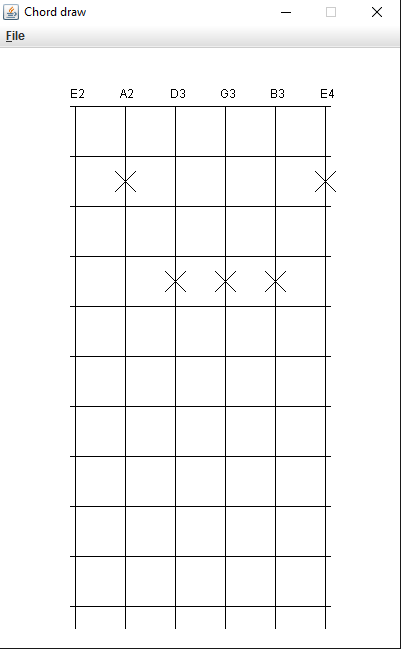
\includegraphics[width=0.5\textwidth]{../img/chords/ChordDraw}
%
% \Subtask Skapa en hjälpmetod \code{cross} som tar in två heltal $x$ och $y$. Metoden ska rita upp ett kryss som är 20x20 pixlar och har sitt centrum i den angivna koordinaten.
%
% \Subtask Rita ut ett kryss där en sträng trycks ner. \textbf{Tänk på att -1 och 0 anger att en sträng inte trycks ner}.
%
% \Subtask Implementera metoden \code{play} som börjar med att vänta på ett event från \code{SimpleWindow}, sedan kollar om eventet är av typen \code{SimpleWindow.MOUSE_EVENT}. Sedan ska man kolla om användaren tryckte på någon sträng (ett intervall på -10 till +10 i förhållande till strängens x-koordinat kan anses vara på strängen). Om användaren tryckt på en sträng ska denna spelas med hjälp av \code{SimpleNotePlayer}. Metoden \code{play} ska köras tills användaren kryssar ner fönstret, vilket motsvarar \code{SimpleWindow.CLOSE_EVENT}.
%
% \Subtask Lägg till menyvalet \code{draw} i \code{textui}. Använd \code{match} för att ta hand om felfallen att inget argument eller fler än ett argument angivits. Argumentet motsvarar ackordets plats i den filtrerade litan. Använd \code{Try} och \code{match} för att ta hand om felet att användaren anger något annat än en siffra. Använd \code{ChordDraw} för att rita upp ackord. \textbf{Kom ihåg att lägga till kommandot i listan med kommandon i \code{doCommand}}
